%! TEX root = main.tex  % Specifies the main document file for multi-file projects

\chapter{SuperCollider ecosystem}

SuperCollider is an engine for sound synthesis and algorithmic music composition. It provides a real-time sound-based object-oriented programming language, making it suitable for various applications such as music and acoustic research, algorithmic composition, dynamic programming, and live audio coding.

\begin{figure}[!htb]
    \centering
    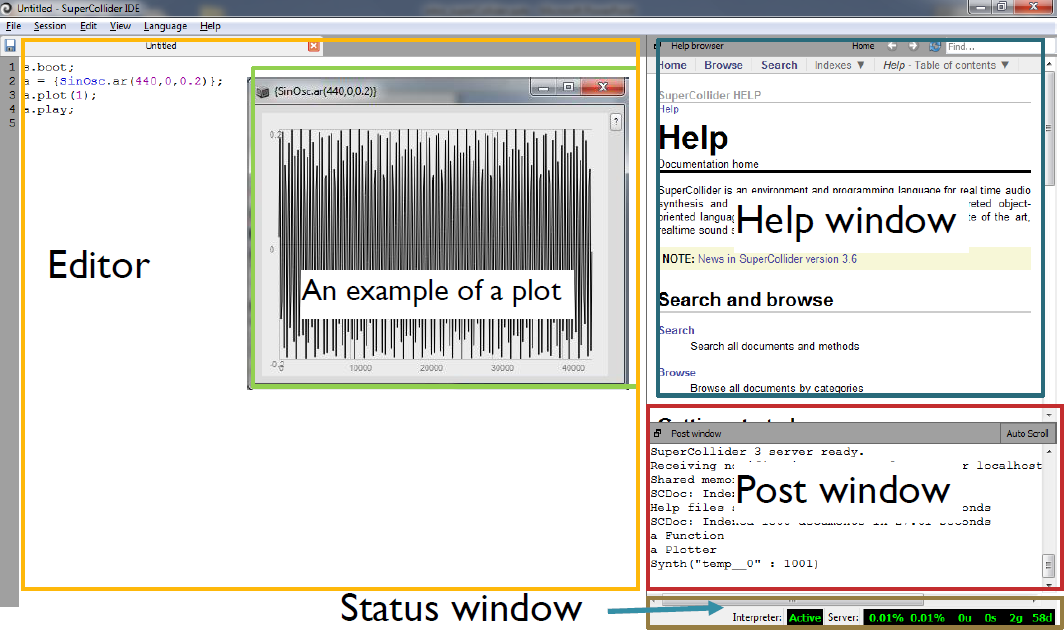
\includegraphics[width=0.8\linewidth]{00_Images/Res/03_chapter/01.png}
    \caption{Appearance of SuperCollider}
    \label{fig:appearance}
\end{figure}

\section{Architecture of SuperCollider}

SuperCollider consists of two main components: a server (scsynth) and a client (sclang), which communicate through OSC (OpenSound Control) messages using TCP/UDP protocols. Additionally, it includes an Integrated Development Environment (IDE).

\subsection{Client and Server}

\begin{itemize}
    \item The server (scsynth) is responsible for sound generation.
    \item The client (sclang) interprets the language and provides a more user-friendly interface.
    \item Typically, both components run on the same machine and communicate via localhost (127.0.0.1), but they can also operate on separate machines.
\end{itemize}

\begin{figure}[!htb]
    \centering
    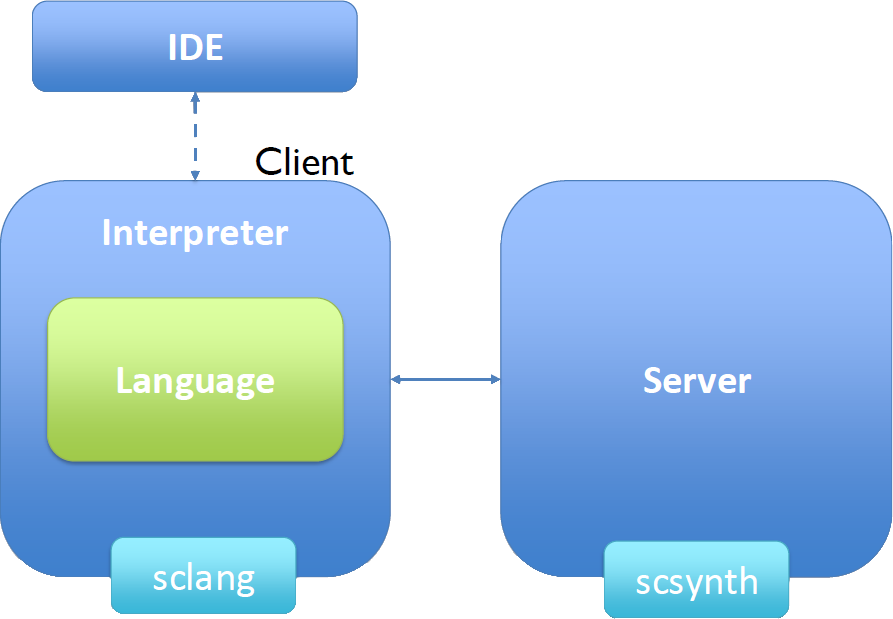
\includegraphics[width=0.5\linewidth]{00_Images/Res/03_chapter/02.png}
    \caption{Interaction between the components}
    \label{fig:interactionserverclient}
\end{figure}

\subsection{Client}

The SC Language (sclang) combines elements of Smalltalk (object-oriented programming) and functional programming. Its syntax follows a C-style structure.

\subsection{Server}

The server is a highly optimized command-line executable, scsynth. Although primarily controlled from within SuperCollider, it can also be used independently. Key features:

\begin{itemize}
    \item Uses OSC for communication.
    \item Supports multiple input and output channels, including large multichannel setups.
    \item Implements a bus system.
    \item Includes buffers for reading and writing.
    \item Operates at three different computation rates: audio rate, control rate, and demand rate.
\end{itemize}

\subsection{SuperCollider IDE}

The Integrated Development Environment (available from version 3.6) includes several components:

\begin{itemize}
    \item Help window.
    \item Post window.
    \item Status window.
    \item Code editor.
    \item Plot visualization tools.
\end{itemize}

SuperCollider is an interpreted language rather than a compiled one. It allows running single lines of code by positioning the cursor on the line and pressing Cmd + Return (MacOS) or Shift + Return (Windows). To stop all server processes, press Cmd + . (MacOS) or Shift + . (Windows).

\subsection{Component Interaction}

SuperCollider's main components interact as follows:

\begin{itemize}
    \item IDE: Provides a graphical user interface.
    \item Interpreter: Executes the SuperCollider language (sclang).
    \item Server (scsynth): Handles audio processing.
    \item Client: Interfaces between the language and the server.
\end{itemize}

\section{The Architecture of the Server}

\subsection{Overview}

The SuperCollider server, scsynth, is an audio synthesis engine that features:

\begin{itemize}
    \item Programmable capabilities.
    \item Real-time audio processing.
\end{itemize}

In scsynth, sound synthesis is achieved through the cooperation of multiple synth objects. The corresponding object in sclang is called Synth. To generate an audio signal, a synth requires processing and synthesis algorithms, which are implemented using UGens (Unit Generators). A UGen is a software module that processes and synthesizes an audio signal. For example, SinOsc is a UGen that generates a sine wave. UGens are the most fundamental components in SuperCollider, analogous to atoms in chemistry. In sclang, items are denoted with uppercase names, whereas in scsynth, their corresponding entities use lowercase names.

\subsection{Synth Creation and UGen Graphs}

To create a new synthesizer, the server requires information about:

\begin{itemize}
    \item The UGens that compose the Synth.
    \item The relationships between these UGens.
\end{itemize}

This information is provided by the client as a UGen graph. In SuperCollider, this is implemented through code, whereas other environments, such as Max/MSP, use graphical representations. A key requirement in SuperCollider is the ability to reuse Synth definitions multiple times. 

\begin{itemize}
    \item The effort to define UGens and their relationships should be done once.
    \item The same Synth structure can be reused with modifications to parameters.
\end{itemize}

For this purpose, SuperCollider provides the SynthDef object, which allows parameter tuning for individual Synth instances.

\begin{figure}[!htb]
    \centering
    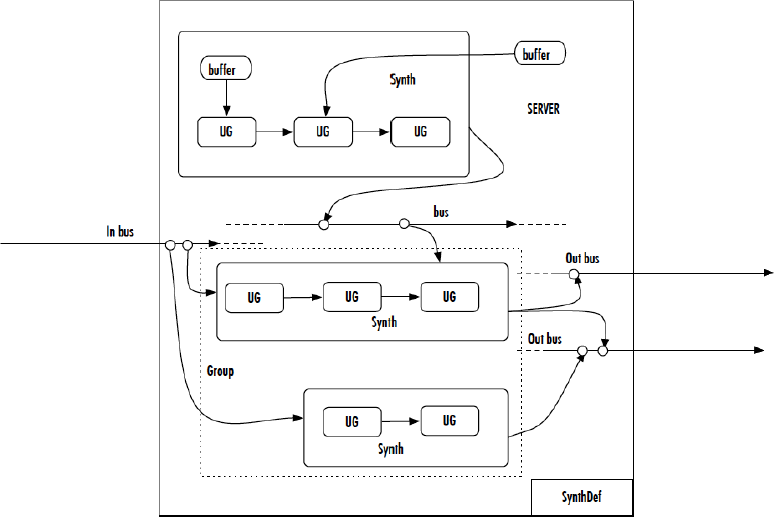
\includegraphics[width=0.8\linewidth]{00_Images/Res/03_chapter/03.png}
    \caption{Example of UGen graph}
    \label{fig:ugengraph}
\end{figure}

\subsection{Synth Communication via Busses}

Multiple Synths interact using busses. Example scenario:

\begin{itemize}
    \item Synth A receives a signal from a microphone and processes it.
    \item The processed signal from Synth A is sent to Bus O.
    \item Synth B retrieves the signal from Bus O, processes it, and sends the output to a special output bus connected to the soundcard.
    \item Synth C processes an audio file and sends the output directly to the output bus.
\end{itemize}

To ensure proper execution, the following conditions must be met:

\begin{itemize}
    \item Synth A must process its signal before Synth B.
    \item Synth A and Synth B must share a private bus that no other Synth can send audio to.
    \item Special busses must be dedicated to input and output signals.
    \item Buffers must be available for reading and writing files.
\end{itemize}

\subsection{Execution Control and Resource Management}

SuperCollider provides mechanisms for:

\begin{itemize}
    \item Controlling the execution order of Synths.
    \item Managing busses for inter-synth communication.
    \item Handling buffers for file operations.
    \item Grouping Synths to manage signal processing workflows.
\end{itemize}

\section{The SuperCollider Language}

\subsection{Object-Oriented Programming in SuperCollider}

SuperCollider follows an object-oriented programming paradigm where:

\begin{itemize}
    \item Objects have properties that can be manipulated.
    \item Objects exchange messages.
    \item Methods define object functionalities for receiving messages and performing operations.
    \item Objects are instances of classes. For example, \texttt{sine1} and \texttt{sine2} can be instances of the \texttt{SinOsc} class, each with different properties despite belonging to the same class.
\end{itemize}

Classes in SuperCollider are organized hierarchically. For example:

\begin{itemize}
    \item \texttt{SinOsc} inherits properties from \texttt{UGen}, a generic signal generator.
    \item Child classes can override parent methods and introduce new properties. For instance, \texttt{SinOsc} adds the \texttt{frequency} property, which \texttt{UGen} does not have.
    \item Some parent class methods can be virtual, meaning they require implementation in child classes.
\end{itemize}

\subsection{Class Notation and Constructors}

\begin{itemize}
    \item Class names start with an uppercase letter. For example, \texttt{Array} is a predefined class for data collections.
    \item Instances of a class are created using constructors. Example:
    
    \begin{supercollider*}
    z = Array.new;
    \end{supercollider*}
    
    \item Some classes have multiple constructors. Example:
    
    \begin{supercollider*}
    z = Array.newClear(indexedSize:12); // Creates an array of 12 elements.
    \end{supercollider*}
    
    \item To check the class of an instance:
    
    \begin{supercollider*}
    z.class;
    \end{supercollider*}
    
    \item To print a class inheritance tree:
    
    \begin{supercollider*}
    Collection.dumpClassSubTree;
    \end{supercollider*}
\end{itemize}

\subsection{Methods and Messages}

Methods in SuperCollider are invoked using the dot notation. Example:

\begin{supercollider*}
z.at(index); // Returns the element at position index.
\end{supercollider*}

To list all methods of a class:

\begin{supercollider*}
ClassName.dumpInterface;
ClassName.dumpFullInterface;
ClassName.dumpMethodList;
\end{supercollider*}

\subsection{Using Methods and Message Chaining}

Example of reversing an array and applying transformations:

\begin{supercollider*}
z = [1,2,3,4];
z.reverse;
z = z.reverse;
z.reverse.mirror.mirror;
\end{supercollider*}

Output:

\begin{supercollider*}
[ 4, 3, 2, 1 ]
[ 1, 2, 3, 4 ]
[ 1, 2, 3, 4, 3, 2, 1, 2, 3, 4, 3, 2, 1 ]
\end{supercollider*}

\subsection{Debugging with postln}

The \texttt{postln} method prints intermediate results:

\begin{supercollider*}
z = [4,3,2,1];
z.postln.reverse.postln.mirror.postln.mirror.postln;
\end{supercollider*}

\subsection{Code Execution and Delimiters}

To execute multiple instructions at once, use parentheses:

\begin{supercollider*}
(
var freq = 440;
SinOsc(freq);
)
\end{supercollider*}

SuperCollider executes one expression at a time, where expressions are delimited by a semicolon.

\subsection{Comments}

\begin{itemize}
    \item Inline comments use \texttt{//}, ignoring text until the end of the line.
    \item Block comments use \texttt{/* */} and can span multiple lines.
\end{itemize}

\subsection{Strings and Variables}

\begin{itemize}
    \item Strings are enclosed in double quotes:
    
    \begin{supercollider*}
    "hello world";
    \end{supercollider*}
    
    \item Variables must be declared, except single-letter variables (\texttt{a-z}).
    \item Local variables are defined using \texttt{var}:
    
    \begin{supercollider*}
    var array = [1,2,3];
    \end{supercollider*}
    
    \item Environment variables use \texttt{\~} instead of \texttt{var}:
    
    \begin{supercollider*}
    ~array = [1,2,3];
    \end{supercollider*}
\end{itemize}

\subsection{Symbols}

Symbols uniquely represent objects:

\begin{supercollider*}
a = \symbol;
b = 'I am a symbol';
a.class;
\end{supercollider*}

\subsection{Functions}

Functions are enclosed in curly brackets:

\begin{supercollider*}
f = { 5 };
f.value; // Returns 5
\end{supercollider*}

Arguments are defined using \texttt{arg}:

\begin{supercollider*}
g = { arg input; input * 2 };
g.value(2); // Returns 4
\end{supercollider*}

Functions can return complex expressions:

\begin{supercollider*}
h = { arg a, b; (a.pow(2) + b.pow(2)).sqrt };
h.value(4,3); // Returns 5
\end{supercollider*}

\subsection{Flow Control}

Example of an if statement:

\begin{supercollider*}
var a = 1, z;
z = if (a < 5, { 100 }, { 200 });
z.postln;
\end{supercollider*}

Example of a while loop:

\begin{supercollider*}
i = 0;
while ( { i < 5 }, { i = i + 1; [i, "boing"].postln });
\end{supercollider*}

Example of a for loop:

\begin{supercollider*}
for (3, 7, { arg i; i.postln });
forBy (0, 8, 2, { arg i; i.postln });
\end{supercollider*}

\subsection{Interacting with the Server}

Basic server commands:

\begin{supercollider*}
s.boot; // Start the server
s.quit; // Stop the server
s.reboot; // Restart the server
\end{supercollider*}

Visualizing signals:

\begin{supercollider*}
s.scope; // Time-domain visualization
s.freqscope; // Frequency-domain visualization
\end{supercollider*}

\subsection{Creating and Controlling Sound}

A simple sinusoidal signal:

\begin{supercollider*}
{ SinOsc.ar(440, 0, 0.2) }.play;
\end{supercollider*}

Modifying amplitude dynamically:

\begin{supercollider*}
(
{ var ampOsc;
  ampOsc = SinOsc.kr(0.5, 1.5pi, 0.5, 0.5);
  SinOsc.ar(440, 0, ampOsc);
}.play;
)
\end{supercollider*}

\subsection{Stereo Output and Panning}

Basic stereo signal:

\begin{supercollider*}
{ [SinOsc.ar(440, 0, 0.2), SinOsc.ar(442, 0, 0.2)] }.play;
\end{supercollider*}

Using multichannel expansion:

\begin{supercollider*}
{ SinOsc.ar([440, 442], 0, 0.2) }.play;
\end{supercollider*}

Randomized frequency selection:

\begin{supercollider*}
(
{ var freq;
  freq = [[660, 880], [440, 660], 1320, 880].choose;
  SinOsc.ar(freq, 0, 0.2);
}.play;
)
\end{supercollider*}

Using Pan2 for panning:

\begin{supercollider*}
{ Pan2.ar(PinkNoise.ar(0.2), SinOsc.kr(0.5)) }.play;
\end{supercollider*}
